	\onecolumn
	\chapter{前言}

	按照考研数学历年的命题规律和风格,结合最新的信息,考生在2020年考研复习备考中应做到以下五点:一是将考研基础知识和常规题目作为复习主体;二是要加强综合性试题的训练;三是加强计算能力的培养,使自己具备较强的处理数学计算过程的本领,要知道,绝大多数数学题都是要通过准确的计算才能得到正确答案的;四是要加强应用能力的培养,多做用数学基础知识解决实际问题的题目;五是要全面复习,将考研大纲中的所有知识作为复习范围,不要有所偏颇。以上五点也将是2020考研命题的趋势,请各位考生重视。

	本书是对题源的最新研究成果,它尽力搜集和命制了题源本身或与题源相关的重要考题,值得考生在复习全过程中认真做题、消化。我也将在各种场合对本书的题目进行详细讲解并予以重点提示,以期让考生把握住考试命题方向,准确复习备考。题源和题库研究是公共资源,从2019年考研命题的情况来看,它并不回避市面上已经公开的题源,甚至可考到原题,于是,我很高兴把我们所掌握的信息提供给全国考生,并乐于与大家分享这些资料。这对消除考研数学的神秘感,进一步促进考试的公正性与科学性都会起到重要作用。

	这本《张宇考研数学题源探析经典1000题》最初是按照数学一、数学二、数学三平均1000道题左右来命名的,多年来一直这样叫下来,成为了考研习题集的一个经典名称。事实上,数学一考试内容最多,题目不止1000道,数学二考试内容最少,题目少于1000道,数学三的考试内容居中,近于1000道。

	衷心感谢原命题专家们给予的指导与帮助。希望考生认真研读、操练本书中的每一道题目,提高解题能力,争取考研得到高分。

	\phantom{1}\hspace{\fill} {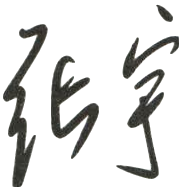
\includegraphics[width=5pc]{figure/fig0.png}}
	
	\phantom{1}\hspace{\fill} {2019 年 2 月\quad 于北京}
	\twocolumn